\documentclass{article}

\usepackage{titlesec}
\usepackage{titling}
\usepackage{graphicx}
\graphicspath{ {writeupimages/} }
\usepackage{float}
\usepackage{amsmath}

\titleformat{\section}
{\Large\bfseries}
{}
{0em}
{}[\titlerule]

\titleformat{\subsection}
{\large\bfseries}
{}
{0em}
{}

\titleformat{\subsubsection}
{\bfseries}
{}
{0em}
{}

\begin{document}

\title{Project: Kinematics Pick \& Place}
\author{Brett Gleason}

\maketitle

The rubric for this project can be found at the following URL: \\
https://review.udacity.com/\#!/rubrics/972/view \\
I will consider the rubric points individually and describe how I addressed each point in my implementation.  

\section{Writeup / README}

\subsection{1. Provide a Writeup / README that includes all the rubric points and how you addressed each one.  You can submit your writeup as markdown or pdf.}

You're reading it!

\section{Kinematic Analysis}
\subsection{1. Run the forward\_kinematics demo and evaluate the kr210.urdf.xacro file to perform kinematic analysis of Kuka KR210 robot and derive its DH parameters.}

Using the model of the Kuka KR210 robotic arm in the forward kinematics demo as well as the description of the joints within the URDF file, a schematic diagram of the robot can be drawn.

\begin{figure}[H]
    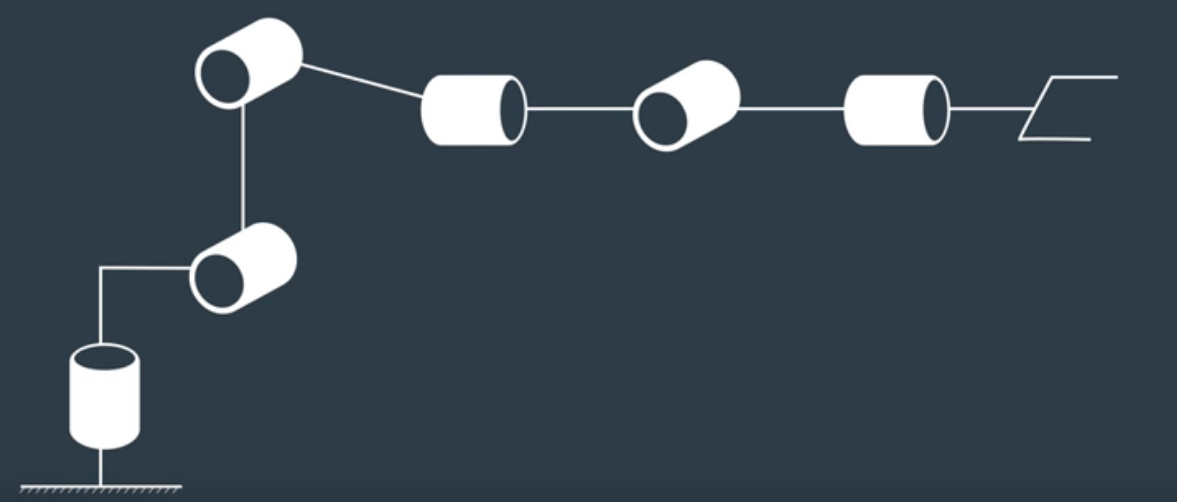
\includegraphics[width=\linewidth]{KR210scheme.png}
    \caption{Basic schematic as shown in project lesson 10}
    \label{fig:scheme}
\end{figure}

Next the joints are labeled from 1 to n and the links are labeled from 0 to n.

\begin{figure}[H]
    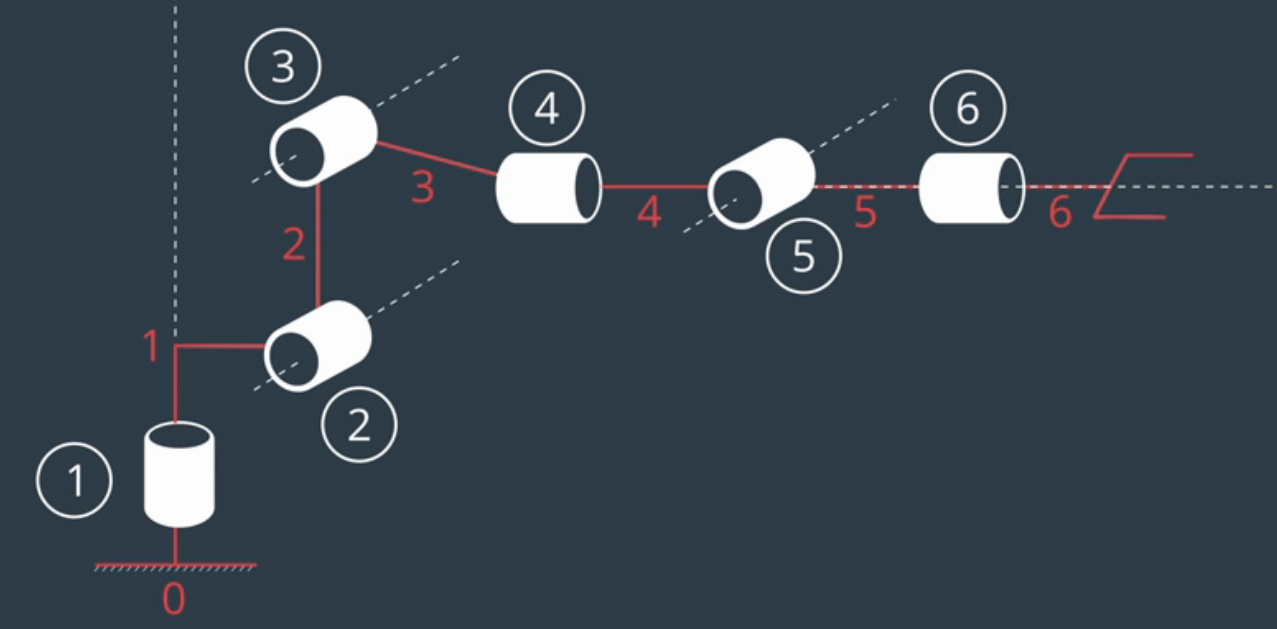
\includegraphics[width=\linewidth]{KR210JL.png}
    \caption{Schematic showing joint and link numbers as shown in project lesson 10}
    \label{fig:JLscheme}
\end{figure}

After the joints and links are labeled, reference frames can be defined for each joint.

\begin{figure}[H]
    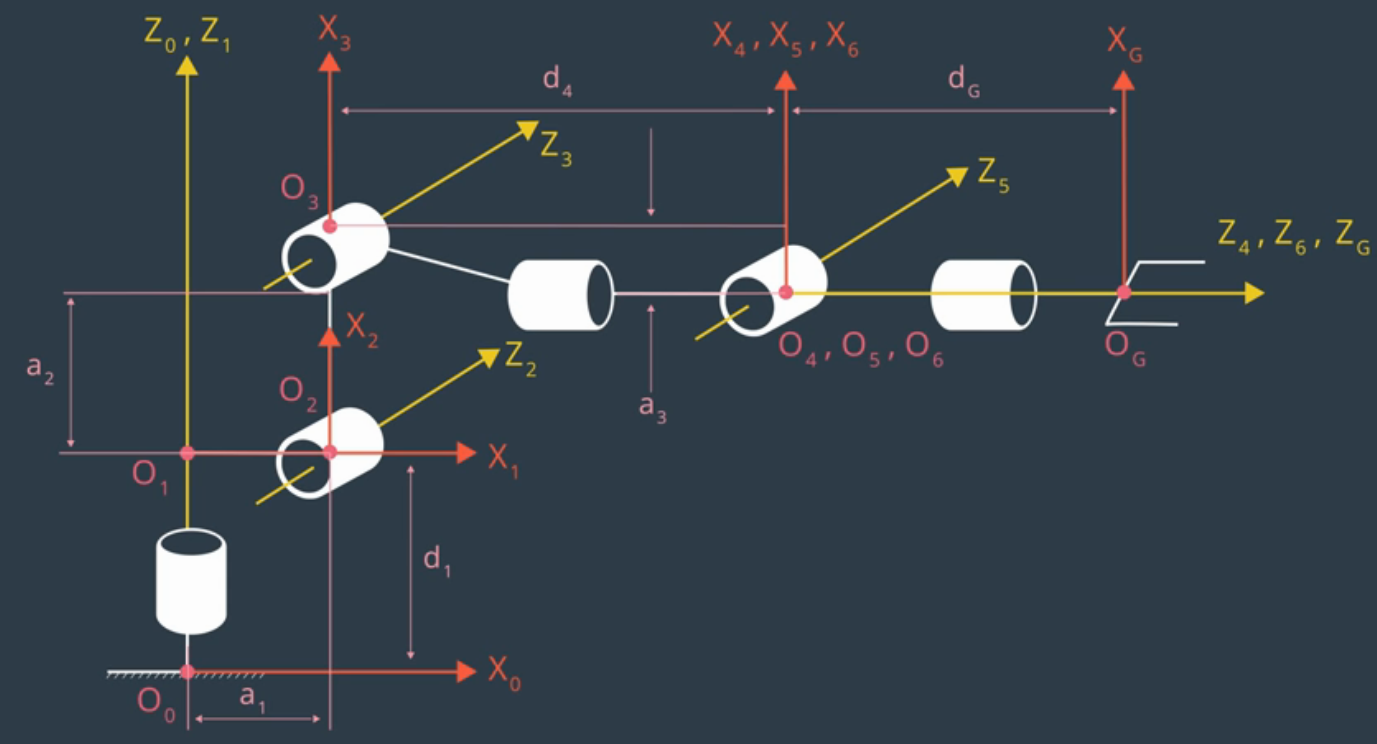
\includegraphics[width=\linewidth]{KR210RF.png}
    \caption{Schematic showing reference frames for each joint as shown in project lesson 10}
    \label{fig:RFscheme}
\end{figure}

Using the reference frames the Denavit-Hartenberg parameters can be defined. For this project the DH parameters are defined using the convention described by John J. Craig in his book Introduction to Robotics: Mechanics and Control. The definitions are as follows (from lesson 2 section 12):

\begin{itemize}
    \item Twist angle ($\alpha _{i-1}$): angle between $\hat{Z}_{i-1}$ and $\hat{Z}_i$ measured about $\hat{X}_{i-1}$ in a right hand sense.
    \item Link length ($a_{i-1}$): distance from $\hat{Z}_{i-1}$ to $\hat{Z}_i$ measured along $\hat{X}_{i-1}$.
    \item Link offset ($d_i$): signed distance from $\hat{X}_{i-1}$ to $\hat{X}_i$ measured along $\hat{Z}_i$.
    \item Joint angle: angle between $\hat{X}_{i-1}$ and $\hat{X}_i$ measured about $\hat{Z}_i$ in a right hand sense.
\end{itemize}

\begin{table}[H]
\centering
\begin{tabular}{|c|r|c|c|l|}
    \hline
    Transform & $\alpha _{i-1}$ & $a_{i-1}$ & $d_i$ & $\theta _i$ \\ \hline
    $T_1^0$ & 0 & 0 & 0.75 & $\theta _1$ \\ \hline
    $T_2^1$ & $-\frac{\pi}{2}$ & 0.35 & 0 & $\theta _2 - \frac{\pi}{2}$ \\ \hline
    $T_3^2$ & 0 & 1.25 & 0 & $\theta _3$ \\ \hline
    $T_4^3$ & $-\frac{\pi}{2}$ & -0.054 & 1.5 & $\theta _4$ \\ \hline
    $T_5^4$ & $\frac{\pi}{2}$ & 0 & 0 & $\theta _5$ \\ \hline
    $T_6^5$ & $-\frac{\pi}{2}$ & 0 & 0 & $\theta _6$ \\ \hline
    $T_G^6$ & 0 & 0 & 0.303 & 0 \\ \hline

\end{tabular}
\caption{\label{tab:table-name}Denavit-Hartenberg parameter table with values derived from the URDF file}
\end{table}

\subsection{2. Using the DH parameter table you derived earlier, create individual transformation matrices about each joint. In addition, also generate a generalized homogeneous transform between base\_link and gripper\_link using only end-effector(gripper) pose.}

The general form of a homogeneous transform between two reference frames described using our convention can be written as follows:
\[
\begin{bmatrix}
    \cos(\theta _i) & -\sin(\theta _i) & 0 & a_{i-1} \\
    \sin(\theta _i)\cos(\alpha _{i-1}) & \cos(\theta _i)\cos(\alpha _{i-1}) & -\sin(\alpha _{i-1}) & -\sin(\alpha _{i-1})d_i \\
    \sin(\theta _i)\sin(\alpha _{i-1}) & \cos(\theta _i)\sin(\alpha _{i-1}) & \cos(\alpha _{i-1}) & \cos(\alpha _{i-1})d_i \\
    0 & 0 & 0 & 1

\end{bmatrix}
\]

\subsection{3. Decouple Inverse Kinematics problem into Inverse Position Kinematics and inverse Orientation Kinematics; doing so derive the equations to calculate all individual joint angles.}

\subsubsection{Theta 1}
\begin{figure}[H]
    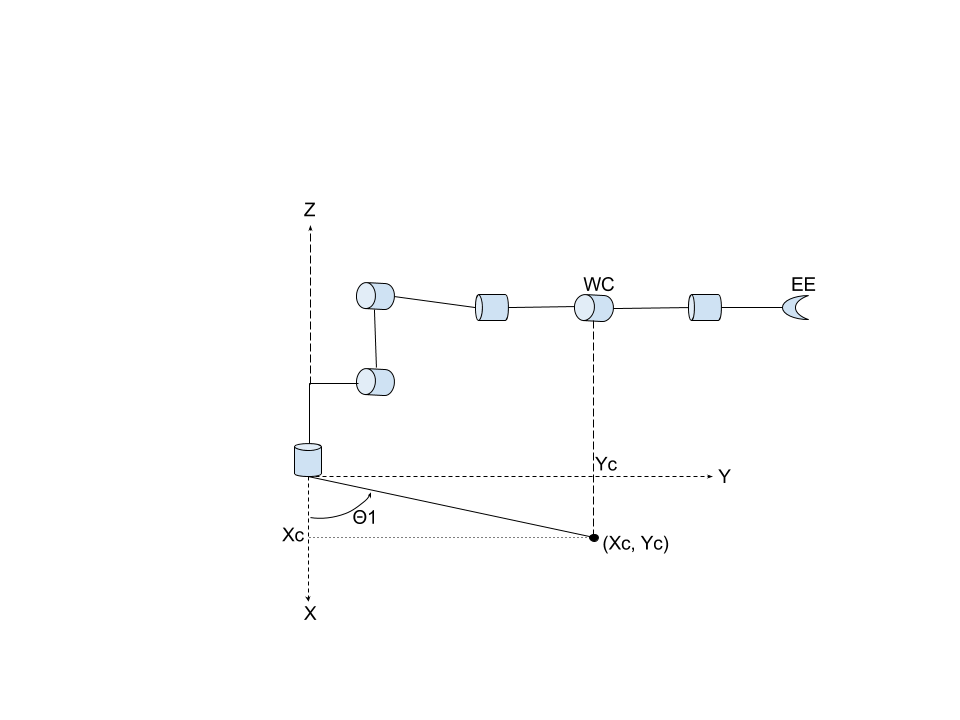
\includegraphics[width=\linewidth]{theta1.png}
    \caption{Diagram for calculating theta 1.}
    \label{fig:theta3}
\end{figure}

\subsubsection{Theta 2}
\begin{figure}[H]
    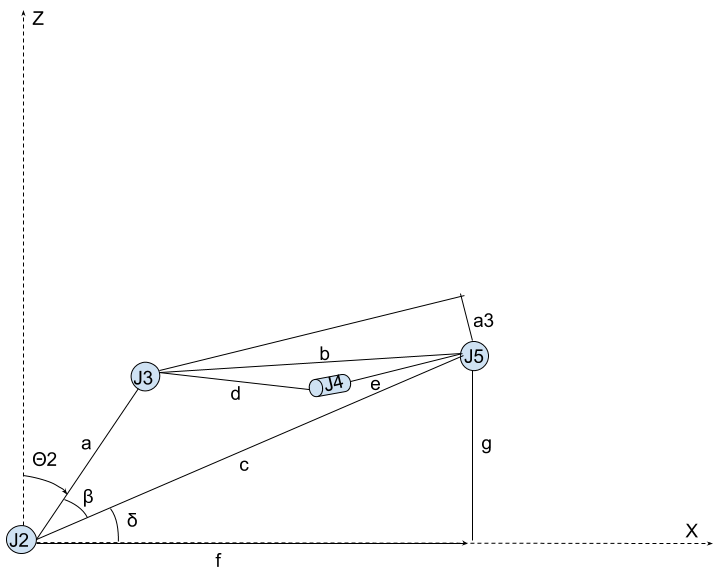
\includegraphics[width=\linewidth]{theta2.png}
    \caption{Diagram for calculating theta 2.}
    \label{fig:theta3}
\end{figure}

\subsubsection{Theta 3}
\begin{figure}[H]
    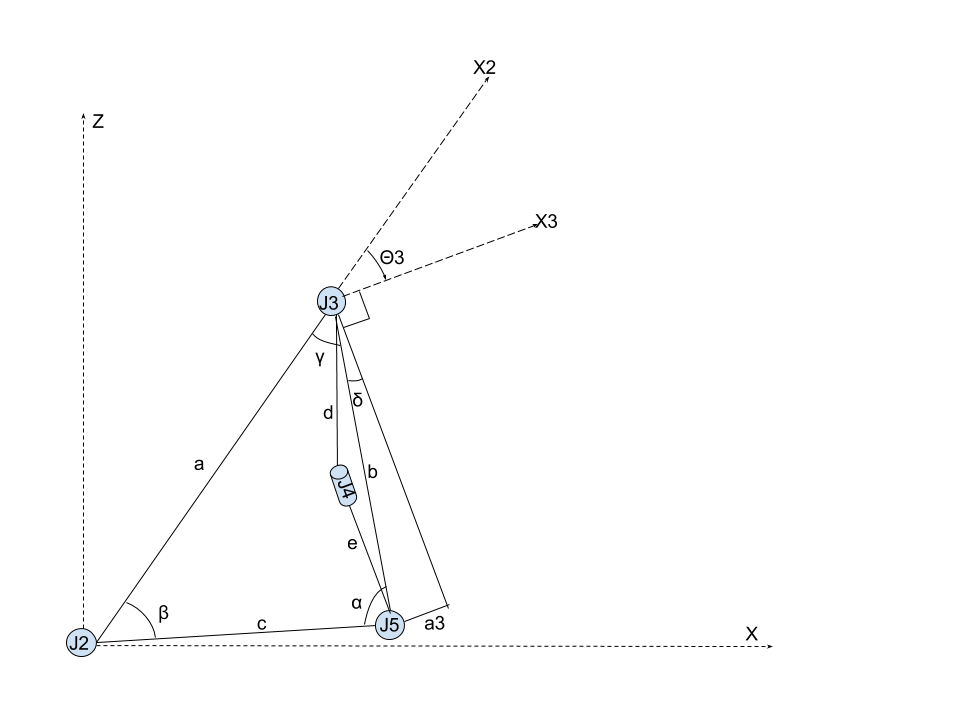
\includegraphics[width=\linewidth]{theta3.png}
    \caption{Diagram for calculating theta 3.}
    \label{fig:theta3}
\end{figure}

\subsubsection{Theta 4}

\subsubsection{Theta 5}

\subsubsection{Theta 6}

\section{Project Implementation}

\subsubsection{1. Fill in the `IK\_server.py` file with properly commented python code for calculating Inverse Kinematics based on previously performed Kinematic Analysis. Your code must guide the robot to successfully complete 8/10 pick and place cycles. Briefly discuss the code you implemented and your results.}


Here I'll talk about the code, what techniques I used, what worked and why, where the implementation might fail and how I might improve it if I were going to pursue this project further.  


And just for fun, another example image:
% ![alt text][image3]

\end{document}
